% !Mode:: "TeX:UTF-8"
\baselineskip=20pt
\cheading{天津大学~2020~届本科生毕业论文}      	% 设置正文的页眉,需要填上对应的毕业年份
\title{他改变了中国:江泽民传}    	% 论文名称
\author{作者}            					% 作者姓名
\email{email: yuyangzhao@outlook.com} %作者邮箱
%%%%%%%%%%%%%如果作者和邮箱过长,可以在format.tex文件中makecover部分取消注释
%\chapter*{中文翻译}
\makecover
\begin{abstract}
\par\setlength{\parindent}{2em} 中文摘要一般在~400~字以内,简要介绍毕业论文的研究目的、方法、结果和结论,语言力求精炼。中英文摘要均要有关键词,一般为~3~—~7~个。字体为小四号宋体,各关键词之间要有分号。英文摘要应与中文摘要相对应,字体为小四号~Times New Roman。
\end{abstract}

\section{第一节}
\subsection{第二级标题}
《他改变了中国:江泽民传》(如图~\ref{book}~所示)这本传记介绍了江泽民同志的人生历程,尤其是阐述和评价了江泽民同志担任中国主要领导人的10多年中创立的历史功绩。在着重于国事活动的同时,也广泛涉及家庭生活、业余爱好、人品风格等方方面面,多角度、多侧面地展现了传主的风采。

\begin{figure}[htbp!]
	\centering
	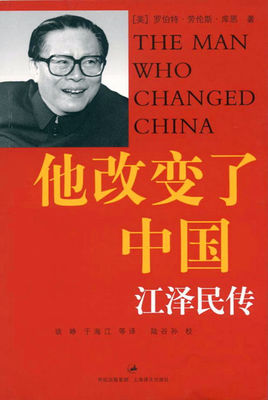
\includegraphics[width=0.5\textwidth]{figures/The_Man_Who_Changed_China.png}
	\caption{红宝书封面}\label{book}
	\vspace{-1em}
\end{figure}	

\begin{table}[htbp]
	\caption{长者用语对照表}\label{table}
	\vspace{0.5em}\centering\wuhao
	\begin{tabular}{ccccc}
		\toprule[1.5pt]
		原文 & 翻译 \\
		\midrule[1pt]
		吼哇 & 好啊 \\
		姿瓷 & 支持 \\
		姿势水平 & 知识水平 \\
		图样 & too young \\
		图森破 & too simple \\
		上台拿衣服 & sometimes naive \\
		识得唔识得啊 & 知道不知道啊 \\
		捉鸡 & 着急 \\
		这是坠吼滴 & 这是最好的 \\
		安格瑞 & angry \\
		一颗赛艇 & excited \\
		\bottomrule[1.5pt]
	\end{tabular}
	\vspace{\baselineskip}
\end{table}


\section{三件小事}
到了北京我干了这十几年也没有什么别的,大概三件事:

\begin{itemize}
	\item 一个,确立了社会主义市场经济;
	\item 第二个,把邓小平的理论列入了党章;
	\item 第三个,就是我们知道的“三个代表”。
\end{itemize}

\section{结论}
我们党要始终代表中国先进生产力的发展要求——就是党的理论、路线、纲领、方针、政策和各项工作,必须努力符合生产力发展的规律,体现不断推动社会生产力的解放和发展的要求,尤其要体现推动先进生产力发展的要求,通过发展生产力不断提高人民群众的生活水平;

我们党要始终代表中国先进文化的前进方向——就是党的理论、路线、纲领、方针、政策和各项工作,必须努力体现发展面向现代化、面向世界、面向未来的,民族的科学的大众的社会主义文化的要求,促进全民族思想道德素质和科学文化素质的不断提高,为我国经济发展和社会进步提供精神动力和智力支持;

我们党要始终代表中国最广大人民的根本利益——就是党的理论、路线、纲领、方针、政策和各项工作,必须坚持把人民的根本利益作为出发点和归宿,充分发挥人民群众的积极性主动性创造性,在社会不断发展进步的基础上,使人民群众不断获得切实的经济、政治、文化利益。
